%% Type de document et encodage de la police
\documentclass[a4paper]{article}
\usepackage[utf8x]{inputenc}
\usepackage[T1]{fontenc}
% \usepackage[french]{babel}

%% Initialise la taille des pages et des marges
\usepackage[a4paper, top=3cm, bottom=3cm, left=2cm, right=2cm, marginparwidth=2cm]{geometry}

%% Packs utiles
\usepackage{amsmath}
\usepackage{graphicx}
\usepackage{array}

%% Commandes perso
\renewcommand{\arraystretch}{1.2} %% row 20% longer
\newcolumntype{C}[1]{>{\centering\let\newline\\\arraybackslash\hspace{0pt}}m{#1}}

%% Pour les exemples
\usepackage{mdframed}
\newmdenv[topline=false, bottomline=false, rightline=false, skipabove=\topsep, skipbelow=\topsep]{example}

%% Pour les diagrammes
\usepackage{tikz}
\tikzstyle{incolore} = [rectangle, rounded corners, draw=black, minimum height=1cm, minimum width=3cm, text width=3cm, text centered]


\title{Réseaux Applicatifs - Théorie}
\author{Grégoire Roumache}
\date{Janvier 2020}

\begin{document}

\maketitle















\section{Introduction}





\begin{itemize}





\item Caractéristiques des architectures de réseaux:
\begin{itemize}
    \item fault tolerance (= tolérance aux pannes),
    \item scalability (= capable de grandir),
    \item quality of service,
    \item security.
\end{itemize}





\item Types de réseaux:
\begin{itemize}
    \item Local Area Networks (\textbf{LAN})
    \begin{example}
        % Ex: un réseau dans une maison, un immeuble, un campus, etc. \\
        L'appareil représentatif du LAN est le \textbf{switch} qui connecte les appareils entre eux.
    \end{example}
    % \item Metropolitan Area Network (\textbf{MAN})
    \item Wide Area Networks (\textbf{WAN})
    \begin{example}
        % Ex: les LAN connectés entre eux et séparés par de longues distances sont des WAN. \\
        L'appareil représentatif du WAN est le \textbf{routeur} qui connecte les réseaux entre eux.
    \end{example}
    \item Internet (interconnected networks) est un ensemble de réseaux interconnectés au niveau mondial.
    \item Metropolitan Area Network (MAN) est un réseau de la taille d'une ville.
\end{itemize}





\item Modèles OSI et TCP/IP:
\begin{center}
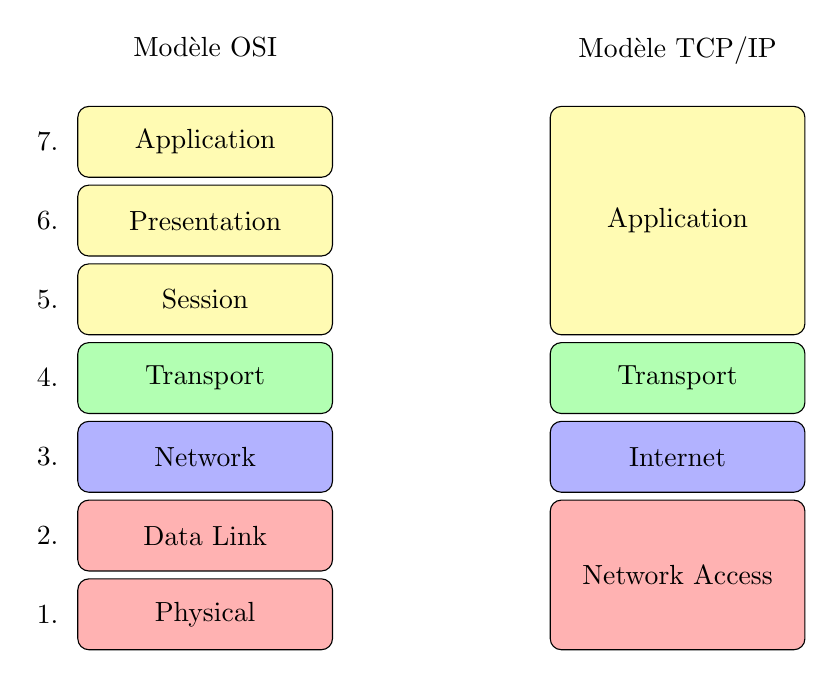
\begin{tikzpicture}
    \node [anchor=north] at (0,0) {Modèle OSI};
    \node [anchor=north] at (6,0) {Modèle TCP/IP};

    \node [incolore, anchor=north, minimum height=0.9cm, fill=yellow!30] at (0,-1) {Application};
    \node [incolore, anchor=north, minimum height=0.9cm, fill=yellow!30] at (0,-2) {Presentation};
    \node [incolore, anchor=north, minimum height=0.9cm, fill=yellow!30] at (0,-3) {Session};
    \node [incolore, anchor=north, minimum height=0.9cm, fill=green!30] at (0,-4) {Transport};
    \node [incolore, anchor=north, minimum height=0.9cm, fill=blue!30] at (0,-5) {Network};
    \node [incolore, anchor=north, minimum height=0.9cm, fill=red!30] at (0,-6) {Data Link};
    \node [incolore, anchor=north, minimum height=0.9cm, fill=red!30] at (0,-7) {Physical};

    \foreach \i in {1,...,7}
    {
        \node [anchor=north, minimum height=0.9cm] at (-2, -8+\i) {\i.};
    }

    \node [incolore, anchor=north, minimum height=2.9cm, fill=yellow!30] at (6,-1) {Application};
    \node [incolore, anchor=north, minimum height=0.9cm, fill=green!30] at (6,-4) {Transport};
    \node [incolore, anchor=north, minimum height=0.9cm, fill=blue!30] at (6,-5) {Internet};
    \node [incolore, anchor=north, minimum height=1.9cm, fill=red!30] at (6,-6) {Network Access};
\end{tikzpicture}
\end{center}





\item Avantages liés à l'utilisation d'un modèle en couches:
\begin{itemize}
    \item aide à la conception de protocole,
    \item favorise la concurrence,
    \item les changements dans une couche n'affectent pas les autres couches,
    \item fournit un langage commun.
\end{itemize}





\end{itemize}















\section{Couche Applicative}





\begin{itemize}





\item La couche application fournit l'interface entre les applications/utilisateurs et le réseau.





\item Protocoles de résolution des noms:
\begin{itemize}
    \item NetBIOS (= nom d'hôte dans les réseaux Microsoft),
    % \begin{example}
    %     Nom NetBIOS = nom d'hôte dans les réseaux Microsoft. \\
    %     Comportement par défaut de la résolution des noms:
    %     \begin{enumerate}
    %         \item cache local,
    %         \item fichier LMHOST,
    %         \item serveur WINS (= Windows Internet Name Service).
    %     \end{enumerate}
    % \end{example}
    \item DNS (= Domain Name Service).
    % \begin{example}
    %     DNS = Domain Name Service \\
    %     Comportement par défaut de la résolution des noms:
    %     \begin{enumerate}
    %         \item cache local,
    %         \item fichier HOST,
    %         \item serveur DNS.
    %     \end{enumerate}
    % \end{example}
\end{itemize}
Objectif = résoudre des noms de domaines en IP (et inversement).





\item Structure du système DNS:
\begin{center}
\includegraphics[width=0.75\textwidth]{images/internet-images-dnsarb.png}
\end{center}
\begin{itemize}
    \item Le système DNS s'appuie sur une structure arborescente.
    \item Chaque noeud est un domaine et possède une étiquette (label).
    \item Chaque feuille (extrémité d'une branche) est un hôte.
    \item Le nom correspondant au chemin d'un hôte jusqu'à la racine est l'\textbf{adresse FQDN}.
    \item Chaque domaine possède un serveur DNS.
    \item Chaque serveur DNS est déclaré dans un DNS de niveau directement supérieur.
    \item Chaque entité est responsable de la gestion de son nom de domaine.
\end{itemize}
Remarque: TLD = Top Level Domain.





\item Types d'enregistrements DNS:





\end{itemize}





\begin{center}
\begin{tabular}{|c|c|c|} \hline
Enregistrement & Signification du nom & Fonction \\ \hline
A & Adresse IPv4 & nom de domaine $ \implies $ IPv4 \\
AAAA & Adresse IPv6 (4$\times$ la taille d'une IPv4) & nom de domaine $ \implies $ IPv6 \\
CNAME & Nom Canonique & nom de domaine $ \implies $ nom de domaine \\
MX & Mail Exchanger & nom de domaine $ \implies $ liste de serveurs (= hôtes) \\
NS & Name Server & délègue la gestion d'une zone à un autre serveur DNS \\ \hline
\end{tabular}
\end{center}

% Exemples:
% \begin{itemize}
%     \item Type A: \texttt{www.example.com} $ \rightarrow $ \texttt{192.168.1.32}
%     \item Type AAAA: \texttt{www.example.com} $ \rightarrow $ \texttt{2a02:a03f:417b:3300:3c88:a5ee:451b:82ca}
%     \item Type CNAME: \texttt{www.hotmail.com} $ \rightarrow $ \texttt{www.outlook.com}
%     \item Type MX:
%     \begin{itemize}
%         \item mail: \texttt{greg@example.com}
%         \item nom de domaine: \texttt{example.com}
%         \item hôtes: \texttt{server1.example.com}, \texttt{serveur2.example.com}, etc.
%     \end{itemize}
%     \item Type NS:
%     \begin{center}
%         \includegraphics[width=0.65\textwidth]{images/zone-microsoft.PNG}
%     \end{center}
%     La zone: \texttt{microsoft.com}, contient un enregistrement NS qui délègue la gestion de la zone: \\ \texttt{example.microsoft.com}, à un autre serveur DNS.
% \end{itemize}





\begin{itemize}





\item Types de zones \& serveurs DNS:
\begin{itemize}
    \item zone maître (Master ou Primary),
    \item zone esclave (Slave ou Secondary),
    \item zone cache (caching),
    \item zone inverse (Reverse),
    \item serveur forwarder.
\end{itemize}





\item Le DNS utilise le port 53 et les protocoles TCP et UDP:
\begin{itemize}
    \item UDP pour les requêtes,
    \item TCP pour la synchronisation entre zones.
\end{itemize}





\item 3 types de requêtes DNS: itératives, récursives, inverses.
\begin{itemize}
    \item itérative = demande la meilleure réponse possible (y compris partielle) -- typique d'un serveur
    \item récursive = réponse obligatoire soit correcte et complète, soit négative -- typique d'un client
\end{itemize}





\item Types de réponses DNS:
\begin{itemize}
    \item autoritative: réponse d'un serveur qui gère la zone concernant la requête.
    \item non-autoritative: réponse d'un serveur qui connaît la réponse via le mécanisme de cache.
\end{itemize}





\item Fonctionnement protocole HTTP (port 80, https = port 443):
\begin{enumerate}
    \item le client effectue une requête http,
    \item le serveur répond avec le code html demandé,
    \item le client interprète le code html et formate/affche la page,
    \item la session est terminée.
\end{enumerate}





\item DHCP est un protocole qui assure la configuration automatique des paramètres IP. Avantages:
\begin{itemize}
    \item gestion des IP centralisée et simplifiée,
    \item partage optimisé des adresses disponibles,
    \item évite les conflits IP,
    \item portable et universel: idéal pour assigner des paramètres aux clients mobiles.
\end{itemize}





\item Étapes du cycle de vie DHCP:
\begin{enumerate}
    \item affectation: acquisition des paramètres par le client,
    \item réallocation: le client redemande au serveur ses paramètres toujours valides,
    \item opérations "normales": utilisation des paramètres fournis,
    \item renouvellement: le client tente de renouveler son bail,
    \item réafectation: le client tente de renouveler son bail auprès d'un autre serveur si l'ancien est injoignable,
    \item libération: le client libère le bail.
\end{enumerate}





\item Les messages DHCP:
\begin{itemize}
    \item DHCP DISCOVER = diffusion du client pour localiser les serveurs disponibles.
    \item DHCP OFFER = réponse du serveur avec les paramètres de configuration.
    \item DHCP REQUEST = message client (3 possibilités):
    \begin{enumerate}
        \item qui demande les paramètres à un serveur.
        \item qui confirme la validité des adresses précédemment allouées.
        \item qui étend le bail sur une adresse réseau en particulier.
    \end{enumerate}
    \item DHCP ACK = message du serveur avec les paramètres de configuration.
    \item DHCP NACK = message du serveur indiquant que le bail a expiré.
    \item DHCP DECLINE = message du client indiquant que l'adresse réseau est déjà utilisée.
    \item DHCP RELEASE = message du client libérant l'adresse réseau et annulant le bail.
\end{itemize}
Remarque: DHCP REQUEST est utilisé lors de l’affectation, du renouvèlement et de la réaffectation.





\item Les protocoles mail:
\begin{itemize}
    \item SMTP (= Simple Mail Transfer Protocol), port = 25
    \item POP3 (= Post Office Protocol), port = 110
    \item IMAP (= Internet Message Access Protocol), port = 143
    \item SMTPS, POPS, IMAPS
\end{itemize}





\item Agents de messagerie:
\begin{itemize}
    \item MDA = Mail Delivery Agent
    \item MUA = Mail User Agent
    \item MTA = Mail Transfer Agent
\end{itemize}





\item Envoi d'un email:
\begin{center}
\begin{tikzpicture}
    \node (expediteur) [] at (0,0) {\includegraphics[width=1.5cm]{images/laptop.jpg}};
    \node (destinataire) [] at (7,0) {\includegraphics[width=1.5cm]{images/laptop.jpg}};

    \node (server1) [] at (0,4) {\includegraphics[height=1.5cm]{images/server.jpg}};
    \node (server2) [] at (7,4) {\includegraphics[height=1.5cm]{images/server.jpg}};

    \node [below of = expediteur, text width=3cm, text centered, anchor=north] {Expéditeur \\ \textbf{MUA}};
    \node [below of = destinataire, text width=3cm, text centered, anchor=north] {Destinataire \\ \textbf{MUA}};
    \node [above of = server1, text width=3cm, text centered, anchor=south] {Serveur \\ \textbf{MTA}};
    \node [above of = server2, text width=3cm, text centered, anchor=south] {Serveur \\ \textbf{MDA}};

    \draw [->, red, thick] (expediteur) -- node[anchor=east]{SMTP} (server1);
    \draw [->, red, thick] (server1) -- node[anchor=south]{SMTP} (server2);
    \draw [->, red, thick] (server2) -- node[anchor=west]{POP} (destinataire);
\end{tikzpicture}
\end{center}





\item Fonctionnement de POP3:
\begin{enumerate}
    \item connexion au serveur,
    \item téléchargement des fichiers,
    \item effacement des fichiers sur le serveur.
\end{enumerate}





\item Autre protocole de réception de mail, \textbf{IMAP}:
\begin{itemize}
    \item les dossiers manipulés (contenant les mails) ne sont pas locaux mais sur le serveur,
    \item les manipulation (ex: suppression de mail) sont donc répercutées sur le serveur,
    \item des copies locales sont toujours possibles.
\end{itemize}





\item Protocole de transfert de fichier, \textbf{FTP} (= File Transfer Protocol):
\begin{itemize}
    \item fiable,
    \item performant,
    \item versions sécurisées: SFTP, FTPS,
    \item port 21 = commande et réponses,
    \item port 20 = transfert de fichiers.
\end{itemize}





\item Protocole TFTP (= Trivial File Transfer Protocol):
\begin{itemize}
    \item port 69,
    \item version simplifiée de FTP:
    \begin{itemize}
        \item UDP au lieu TCP,
        \item pas de listing de fichier ou dossiers,
        \item pas d'authentification,
        \item pas de chiffrement,
    \end{itemize}
\end{itemize}





\end{itemize}















\section{Couche Réseaux}





\begin{itemize}





\item Caractéristiques du protocole IP (= Internet Protocol):
\begin{enumerate}
    \item sans connection,
    \item au mieux (non fiable),
    \item indépendant du média.
\end{enumerate}
Remarque: le protocole IP n'est pas fiable, mais d'autres protocoles gèrent le processus de suivi des paquets (ex: TCP).





\item Avantages de créer des sous-réseaux:
\begin{enumerate}
    \item plus facile à administrer,
    \item plus performant,
    \item augmente la sécurité,
    \item l'adressage est hiérarchisé: réseau -- sous-réseau -- hôte.
\end{enumerate}





\item Routeur v.s. Switch:
\begin{center}
\begin{tabular}{|c|C{2cm}|C{2cm}|} \hline
    & Routeur & Switch \\ \hline
    vitesse & lent & rapide \\
    couche OSI & couche 3 & couche 2 \\
    adressage utilisé & IP & MAC \\
    broadcast & bloqués & transmis \\
    sécurité & élevée & faible \\ \hline
\end{tabular}
\end{center}





\item Une \textbf{route} a 3 composants:
\begin{itemize}
    \item le réseau de destination,
    \item le masque,
    \item le gateway.
\end{itemize}
Notation d'une route: \texttt{<réseau>/<masque> via <ip\_gateway>}.





\end{itemize}















\section{Couche Transport}





\begin{itemize}





\item Quand un serveur exécute plusieurs services (ex: mail \& www), il sait quels paquets sont destinés à quels services grâce aux numéros de port.





\item Quand un client ouvre plusieurs sessions sur un même serveur, le serveur distingue les sessions en attribuant à chacune un numéro de port différent.





\item Fonctionnalités communes TCP/UDP:
\begin{itemize}
    \item segmentation,
    \item multiplexage,
    \item contrôle d'erreur.
\end{itemize}





\item Fonctionnalités de TCP:
\begin{itemize}
    \item fiabilité
    \begin{example}
        \begin{itemize}
            \item accusés de réception
            \item retransmission des segments perdus
        \end{itemize}
    \end{example}
    \item délivre les données dans le bon ordre
    \begin{example}
        \begin{itemize}
            \item segmente
            \item numérote
            \item réassemble
        \end{itemize}
    \end{example}
    \item orienté connexion
    \begin{example}
        \begin{itemize}
            \item session TCP (3-way handshake)
        \end{itemize}
    \end{example}
    \item contrôle de flux
    \begin{example}
        \begin{itemize}
            \item fenêtre glissante
            \item garde une trace de la connexion
        \end{itemize}
    \end{example}
\end{itemize}





\item Étapes d'une session TCP:
\begin{enumerate}
    \item établissement de la session,
    \item session,
    \item fin de la session.
\end{enumerate}





\item Les flags TCP:
\begin{itemize}
    \item SYN = ouverture de session,
    \item ACK = accusé de réception,
    \item FIN = fermeture de session.
\end{itemize}





\item Autres éléments importants du header TCP:
\begin{itemize}
    \item sequence number = le numéro du premier octet de données du segment,
    \item acknowledgement number = le numéro du prochain octet (segment) attendu par le récepteur.
\end{itemize}





\item Remarques:
\begin{itemize}
    \item Full duplex $ \implies $ périphérique = émetteur \& récepteur.
    \item Si un segment envoyé ne reçoit pas d'acknowledgement après un certain temps, il est renvoyé.
    \item Ni TCP, ni UDP ne sont sécurisés.
    \item \textbf{TCP} est \textbf{fiable}.
    \item \textbf{UDP} est \textbf{rapide}.
\end{itemize}





\end{itemize}










\end{document}
